
%(BEGIN_QUESTION)
% Copyright 2009, Tony R. Kuphaldt, released under the Creative Commons Attribution License (v 1.0)
% This means you may do almost anything with this work of mine, so long as you give me proper credit

Beregning av gasstrøm gjennom en reguleringsventil er noe mer kompleks enn beregning av væskestrøm. En standard ligning for gasstrøm gjennom en ventil, forutsatt fravær av kvelning (sonisk, eller {\it kritisk}, gasshastighet i ventilen), er følgende:

$$Q = 963 \> C_v \sqrt{{\Delta P (P_1 + P_2)} \over {G_g T}}$$

\noindent
Hvor,

$Q$ = Gasstrømningsrate, i enheten Standard Cubic Feet per Hour (SCFH)

$C_v$ = Ventilens kapasitetskoeffisient

$\Delta P$ = Trykkfall over ventilen, pounds per square inch differential (PSID)

$P_1$ = Oppstrøms ventiltrykk, pounds per square inch absolute (PSIA)

$P_2$ = Nedstrøms ventiltrykk, pounds per square inch absolute (PSIA)

$G_g$ = Gassens spesifikke vekt (luft ved standard temperatur og trykk = 1.0)

$T$ = Absolutt gasstemperatur i grader Rankine ($^{o}$R)

\vskip 10pt

Bruk denne ``subkritiske'' formelen for gasstrøm gjennom ventil, og bestem hvor stor luftstrøm som går gjennom denne ventilen når den står helt åpen:

$$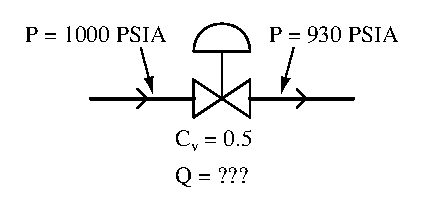
\includegraphics[width=15.5cm]{i01412x01.eps}$$

Anta romtemperatur (70$^{o}$ F) for luften som strømmer gjennom ventilen.

\vskip 10pt

Forklar også hvorfor det er viktig å spesifisere korrekt {\it ANSI flange class} når man bestiller en reguleringsventil til denne applikasjonen.

\vskip 20pt \vbox{\hrule \hbox{\strut \vrule{} {\bf Forslag til sokratisk diskusjon} \vrule} \hrule}

\begin{itemize}
\item{} Forklar hvorfor {\it temperatur} er en like viktig variabel som statisk {\it trykk} når man velger riktig ANSI-klasse for rørflenser og ventiler.
\end{itemize}

\underbar{file i01412}
%(END_QUESTION)





%(BEGIN_ANSWER)

$Q$ = 7,689.91 SCFH
 
%(END_ANSWER)





%(BEGIN_NOTES)

$$Q = 963 \> C_v \sqrt{{\Delta P (P_1 + P_2)} \over {G_g T}}$$

$$Q = (963) (0.5) \sqrt{{(1000 - 930) (1000 + 930)} \over {(1) (70 +459.67)}} = 7689.91 \hbox{ SCFH}$$

\vskip 10pt

Denne ligningen for gasstrøm er avledet fra en ligning på side 27 i Hans D. Baumanns bok, {\it Control Valve Primer, a user's guide}, andre utgave. Andre ligninger for gasstrøm finnes, og de er generelt mer komplekse enn denne, fordi de tar hensyn til rørgeometri og andre faktorer i beregningen.

\vskip 10pt

Gitt det høye arbeidstrykket for denne reguleringsventilen, må rør og rørflenser være riktig klassifisert for sikker og pålitelig drift. Det er kritisk at ventilens trykklasse samsvarer med trykklassen til motflensene på rørene.

%INDEX% Final Control Elements, valve: sizing

%(END_NOTES)

